\documentclass[brazil,times,12pt]{abnt}
\usepackage[T1]{fontenc}
\usepackage[utf8]{inputenc}
\usepackage{url}
\usepackage{graphicx}
\usepackage[pdfborder={0 0 0}]{hyperref}
\makeatletter
\usepackage{babel}
\makeatother
\begin{document}

\autor{Pedro Paulo Vezzá Campos}

\titulo{Pesquisa sobre Modens ADSL e Cable Modens}

\comentario{Trabalho apresentado para avaliação na disciplina INE5414, do
curso de Bacharelado em Ciências da Computação, turma 04208, da Universidade   
Federal de Santa Catarina, ministrada pelo professor Carlos Becker Westphall}

\instituicao{Departamento de Informática e Estatística \par Centro
Tecnológico \par Universidade Federal de Santa Catarina}

\local{Santa Catarina - SC, Brasil}

\data{\today}

\capa

\folhaderosto

% \tableofcontents
%\chapter{}
\section*{Introdução}
Com o avanço da penetração do acesso à Internet em lares e empresas pelo mundo,
há uma crescente demanda por maiores taxas de velocidade, sendo necessário o
desenvolvimento de novas tecnologias que visam otimizar o uso da infraestrutura
disponível. Dentro desse aspecto, realizam papel crucial os modens, responsáveis
por transformar um sinal digital em analógico a ser transmitido por um meio
analógico, tal como linhas telefônicas ou cabos de televisão por assinatura e
vice-versa. Essa tarefa é conhecida por modulação e demodulação, o que deu o
nome ao modem (\textbf{mo}dulator-\textbf{dem}odulator).\cite{enwiki:modem}

%\usepackage{graphics} is needed for \includegraphics
\begin{figure}[htp]
\begin{center}
  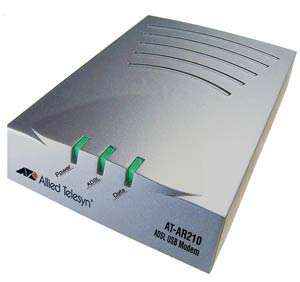
\includegraphics[width=60mm]{imagens/dsl-modem.jpg}
  \caption[Modem ADSL, fonte \cite{hsw:dsl}]{Modem ADSL, fonte \cite{hsw:dsl}}
  \label{modem-adsl}
\end{center}
\end{figure}

Atualmente as empresas que fornecem acesso à Internet podem ser vistas como
``atravessadores'' entre o usuário final e os \emph{backbones} da Internet. O
problema de conectar esses usuários até uma central da empresa é conhecido com o
\textbf{Problema da última milha}. Os modens fornecem parte da solução para esse
problema ao aproveitarem-se da infraestrutura de telefonia ou TV a cabo, por
exemplo para fornecer a conectividade final necessária para o fornecimento do
acesso à Internet. \cite{abusar:ultima-milha}

O avanço do acesso residencial à Internet se deu com a introdução de modens
discados, que aproveitavam-se do sistema de telefonia comutada para a transmissão de dados.
Tanto voz quanto transmissões de dados seguiam numa mesma faixa de frequência
até uma central de telefonia onde eram digitalizados e transmitidos entre centrais
utilizando uma conexão dedicada de 64 kbps. \cite{morimoto:opcoes-acesso} Isso
impôs um limite máximo à velocidade da conexão que foi derrubado com o
desenvolvimento de tecnologias como o ADSL, parte do estudo desse
trabalho.

Comparativamente, há uma disparidade de valores cobrados por acesso de mesma
taxa de velocidade, assinaturas residenciais custam bem menos que uma comercial.
O motivo para isso é que a banda larga residencial
garante normalmente 10\% da banda contratada, com um intenso
\emph{overselling} de recursos na esperança que nem todos os clientes acessem a
Internet ao mesmo tempo. Por outro lado, um \emph{link} dedicado de 1 Mbps em
2000 podia custar entre 1000 e 1500 dólares, necessário para garantir uma
disponibilidade de 100\% da banda contratada. \cite{hsw:t1}

\section*{ADSL}
ADSL ou \emph{Assymmetric Digital Subscriber Line} é uma tecnologia de
transmissão de dados em alta velocidade e grandes distâncias utilizando o
cabeamento existente de telefonia. A grande dificuldade do ADSL é a baixa
qualidade ou idade do cabeamento, este sujeito a menores controles de qualidade
que os cabos categoria 5 ou 6 dos cabeamentos Ethernet.

Diferentemente dos modens discados que transmitiam dados na frequência de 300 Hz
a 3.4 kHz, a mesma dos sinais de voz, o ADSL opera em frequências mais elevadas,
de 26 kHz a 1104 kHz, como é possível ver na figura \ref{espectro-adsl}.

%\usepackage{graphics} is needed for \includegraphics
\begin{figure}[htp]
\begin{center}
  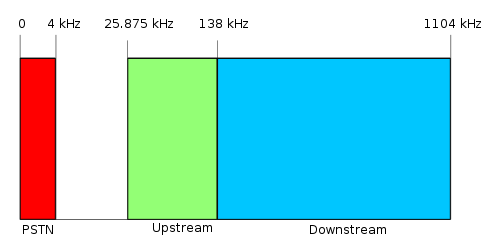
\includegraphics[width=100mm]{imagens/500px-ADSL_frequency_plan.png}
  \caption[Espectro de frequências usadas pelo sistema de
  telefonia e ADSL, fonte \cite{enwiki:adsl}]{Espectro de frequências usadas pelo
  sistema de telefonia e ADSL , fonte \cite{enwiki:adsl}}
  \label{espectro-adsl}
\end{center}
\end{figure}

Essa abordagem incorre no fato de não ocorrer interferência
com o sistema de telefonia, permitindo o funcionamento concomitante de ambos.
Ainda, a especificação original define que a parte baixa do espectro, de 26 kHz
a 138 kHz seja utilizada para \emph{upstream} enquanto o restante seja
aproveitado para \emph{downstream}. A consequência direta disso é que as taxas
de transferência do ADSL são assimétricas, como diz seu nome. O motivo
dessa propriedade é que existe menos ruído do lado da central, do que do lado
do assinante, onde extensões e cabos não utilizados prejudicam a qualidade da
transmissão. Para aumentar a taxa de \emph{downstream} seria necessário
sacrificar grande parte do \emph{downstream}. \cite{morimoto:opcoes-acesso}

As faixas de frequência do ADSL são divididas em canais de 4 kHz. É tarefa do
modem verificar esses canais em busca de seus níveis de atenuação e relação
sinal/ruído, dessa forma podendo isolar os mais problemáticos para garantir um
funcionamento mais adequado. \cite{hsw:dsl}

Ainda, para evitar a contaminação das comunicações de dados por
interferências da comunicação por voz e vice-versa, devem ser instalados
ou um splitter, que divide a linha em duas, uma reservada ao modem ADSL e outra
para os serviços de voz ou então microfiltros, mais baratos, que são conectados
a cada extensão utilizada por aparelhos analógicos.

Graças à modulação e uso de altas frequências, o sinal ADSL pode oferecer taxas
de \emph{downstream} de até 8 Mbps e \emph{upstream} de 1 Mbps para distâncias
entre a residência e a central DSLAM (\emph{Digital Subscriber Line Access
Multiplexer}) de até 2 km, degradando as taxas de transfeerência com o aumento
da distância até um limite de 5 km.

No ADSL há uma conexão contínua (dedicada) entre o modem do assinante e a DSLAM.
Nesta última encontram-se diversos modens ADSL, switch e um roteador que conecta
os assinantes ao backbone da operadora, permitindo o acesso à Internet. 

\subsection*{ADSL2, ADSL2+ e RE-ADSL2+}
O ADSL2 e ADSL2+ são tecnologias mais recentes que aumentaram a taxa de
\emph{downstream} para 12 e 24 Mbps respectivamente. Enquanto o ADSL2 conseguiu
essa façanha sem alterar o espectro de frequência do ADSL original (Figura
\ref{espectro-adsl}) o ADSL2+ utiliza uma faixa mais ampla, de 26 kHz a 2200
kHz, permitindo dobrar a velocidade de seu antecessor. Por outro lado, o
\emph{upstream} permaneceu inalterado em 1 Mbps, o mesmo do ADSL original.

%\usepackage{graphics} is needed for \includegraphics
\begin{figure}[htp]
\begin{center}
  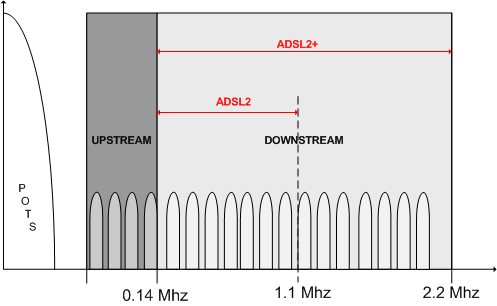
\includegraphics[width=100mm]{imagens/adsl2.png}
  \caption[Espectro de frequências do ADSL2 e ADSL2+, fonte
  \cite{morimoto:opcoes-acesso}]{Espectro de frequências do ADSL2 e ADSL2+,
  fonte \cite{morimoto:opcoes-acesso}}
  \label{espectro-adsl2}
\end{center}
\end{figure}

Os 24 Mbps são obtidos a distâncias de até 1.5 km e decaem para até 4
Mbps em distâncias superiores a 3.6 km. O RE-ADSL2+ vai na direção oposta e
oferece taxas de transferência de até 768 kbps mas permitindo um alcance de até
6 km. \cite{morimoto:opcoes-acesso}

Essas tecnologias possuem compatibilidade com o ADSL original, o que permitiu o
surgimento de modens que aceitam todas as versões da tecnologia, permitindo
baratear custos e facilitar a migração das redes para padrões mais avançados.


\section*{Acesso via Cabo}
Tal como o ADSL, o acesso via cabo reaproveita uma infraestrutura instalada,
utilizando uma faixa do espectro de frequências não utilizada pelos serviços de
televisão a cabo e assim permitindo o uso em paralelo dos dois serviços. Neste
caso, o cabeamento é o coaxial, melhor blindado eletromagneticamente que o de
par trançado das linhas telefônicas.

O acesso via cabo pode atingir maiores frequências, logo
maiores velocidades, graças ao cabeamento de melhor qualidade. Por outro
lado, uma desvantagem é o fato que um único cabo é compartilhado por 100 a 1000
assinantes, assim, as taxas de transferências são divididas entre esses clientes
\cite{morimoto:opcoes-acesso}.

Especificamente no caso do acesso via cabo, o espectro é dividido em canais de 6
MHz com a faixa de \emph{upstream} indo de 5 a 65 MHz e a de \emph{downstream}
de 850 a 1000 MHz como pode ser visto na figura \ref{espectro-cable-modem}.
\cite{hsw:cable-modem}

%\usepackage{graphics} is needed for \includegraphics
\begin{figure}[htp]
\begin{center}
  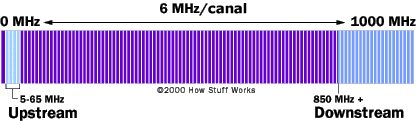
\includegraphics[width=80mm]{imagens/cable-modem-frequency.png}
  \caption[Espectro de frequências do acesso via cabo, fonte
  \cite{hsw:cable-modem}]{Espectro de frequências do acesso via cabo, fonte
  \cite{hsw:cable-modem}}
  \label{espectro-cable-modem}
\end{center}
\end{figure}

O padrão DOCSIS 1.0 atinge a taxa de 10.24 Mbps, já a versão 2.0 aperfeiçoou a
modulação utilizada atingindo taxas de 30 Mbps, por fim, a versão 3.0 prevê
taxas de transferência de 343 Mbps de \emph{downstream} e 122 Mbps de
\emph{upstream}. Os três padrões são intercompatíveis, mais uma vantagem que
leva a empresas a atualizarem suas redes para oferecer serviços de maior
velocidade a seus clientes enquanto reduzem custos já que há uma economia de
banda por \emph{overhead} à medida que novas versões surgem.
\cite{enwiki:docsis} \cite{morimoto:opcoes-acesso}

No papel similar ao DSLAM, há o CMTS (\emph{Cable Modem Termination System}),
responsável por decodificar os sinais enviados pelos cable modens e roteá-los à
Internet. Ainda, uma vez que o cabo é compartilhado por vários clientes, há a
necessidade de criptografar as transmissões para garantir que clientes só se comuniquem com o
CTMS e não entre si. O protocolo usado é o BPI (\emph{Baseline Privacy
Interface}) com uma encriptação de 56 bits.



\bibliographystyle{abnt-num}
\bibliography{bibliografia}
\end{document}